% 卡诺热机
% 卡诺热机|等温过程|绝热过程|热机效率
\pentry{等温过程\upref{EqTemp}, 绝热过程\upref{Adiab},熵\upref{Entrop}}

\subsection{卡诺热机的工作过程}
\textbf{卡诺循环(Carnot cycle)}是一个特别的热力学循环,使用在一个假想的\textbf{卡诺热机}上,由法国人尼古拉·卡诺于1824年提出,埃米尔·克拉佩龙于1830年代至1840年代扩充,是为了找出热机的最大的工作效率而分析热机的工作过程.

\begin{figure}[ht]
\centering
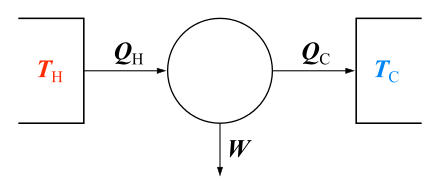
\includegraphics[width=7cm]{./figures/Carnot_1.png}
\caption{热机示意图(来自维基百科)} \label{Carnot_fig1}
\end{figure}
卡诺循环由两个等温过程,两个绝热过程,下面先通过两个图来直观感受一下卡诺热机的工作过程.

压强-体积图,即$P$-$V$图,是大家十分熟悉的:
\begin{figure}[ht]
\centering
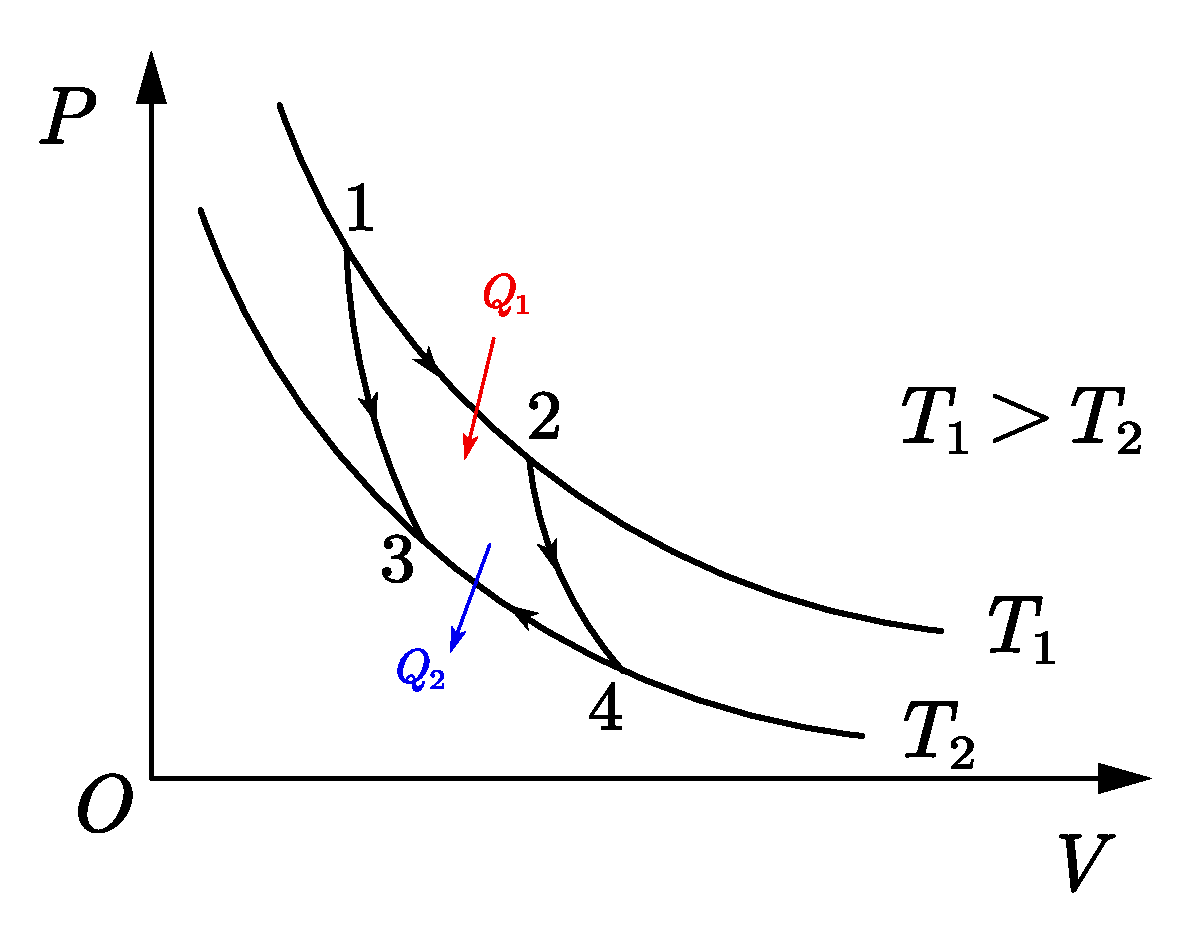
\includegraphics[width=6.5cm]{./figures/Carnot_2.pdf}
\caption{卡诺循环的压强-体积图} \label{Carnot_fig2}
\end{figure}
温度-熵图,即 $T$-$S$ 图,则如下所示:
\begin{figure}[ht]
\centering
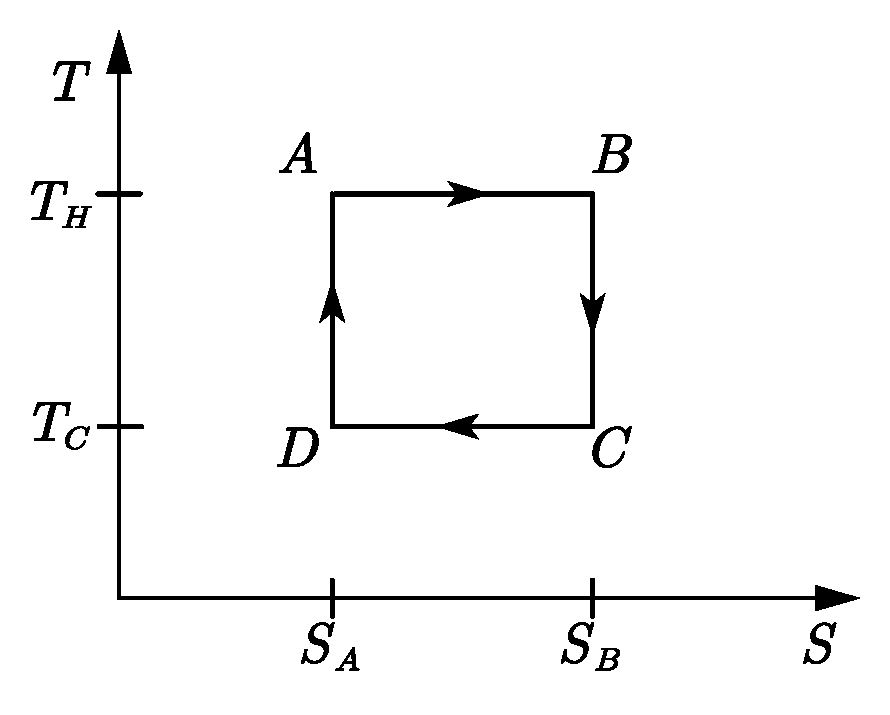
\includegraphics[width=6.5cm]{./figures/Carnot_3.pdf}
\caption{卡诺循环的温度-熵图} \label{Carnot_fig3}
\end{figure}

\autoref{Carnot_fig2} $1\to 2$、\autoref{Carnot_fig3} $A\to B$,可逆等温膨胀:此等温的过程中系统从高温热库吸收了热量且全部拿去做功.

\autoref{Carnot_fig2} $2\to 3$、\autoref{Carnot_fig3} $B\to C$,等熵(可逆绝热)膨胀:移开热库,系统对环境做功,其能量来自于本身的内能.

\autoref{Carnot_fig2} $3\to 4$、\autoref{Carnot_fig3} $C\to D$,可逆等温压缩:此等温的过程中系统向低温热库放出了热量.同时环境对系统做正功.

\autoref{Carnot_fig2} $4\to 1$、\autoref{Carnot_fig3} $D\to A$,等熵(可逆绝热)压缩:移开低温热库,此绝热的过程系统对环境作负功,系统在此过程后回到原来的状态.

\subsection{卡诺循环的效率}

下面我们来分析一下卡诺循环的效率. 气体在等温膨胀过程中,从高温热源吸取热量,
\begin{equation}
Q_{1}=\frac{m}{M} R T_{1} \ln \frac{V_{2}}{V_{1}}
\end{equation}
气休在等温压缩过程中向低温热源放出热量$Q_2$,为便于研究,取绝对值,有
\begin{equation}
Q_{2}=\frac{m}{M} R T_{2} \ln \frac{V_{3}}{V_{4}}
\end{equation}
应用绝热过程方程$T_{1} V_{2}^{\gamma-1}=T_{2} V_{3}^{\gamma-1}$和$T_{1} V_{1}^{\gamma-1}=T_{2} V_{4}^{\gamma-1}$可得
\begin{equation}
\left(\frac{V_{2}}{V_{1}}\right)^{\gamma-1}=\left(\frac{V_{3}}{V_{4}}\right)^{\gamma-1}
\end{equation}
也就是说
\begin{equation}
\frac{V_{2}}{V_{1}}=\frac{V_{3}}{V_{4}}
\end{equation}
所以有
\begin{equation}
Q_{2}=\frac{m}{M} R T_{2} \ln \frac{V_{3}}{V_{4}}=\frac{m}{M} R T_{2} \ln \frac{V_{2}}{V_{1}}
\end{equation}
取$Q_1$与$Q_2$的比值,可得
\begin{equation}
\frac{Q_{1}}{T_{1}}=\frac{Q_{2}}{T_{2}}
\end{equation}
因此卡诺热机的效率为
\begin{equation}
\eta_{\mathrm{c}}=1-\frac{Q_{2}}{Q_{1}}=1-\frac{T_{2}}{T_{1}}
\end{equation}

卡诺热机有几条重要性质,我们做个总结.

\begin{enumerate}
\item 要完成一次卡诺循环必须有高温和低温两个热源;
\item 卡诺循环的效率只与两个热源的温度有关,高温热源的温度越高,低温热源的温度越低,卡诺循环的效率越大,也就是说节两热源的温度差越大,从高温热源所吸取的热量$Q_1$的“利用价值”越大;
\item 卡诺循环的效率总足小于$1 $的.
\end{enumerate}

实际上,卡诺循环还有个逆循环过程,功能应该都可以猜到,也就是制冷机.通过类似对卡诺循环的分析,可以得到制冷系数
\begin{equation}
w_{\mathrm{C}}=\frac{Q_{2}}{A}=\frac{Q_{2}}{Q_{1}-Q_{2}}=\frac{T_{2}}{T_{1}-T_{2}}
\end{equation}

\begin{example}{卡诺制冷机}
有一卡诺制冷机,从温度为$-10^{\circ} \mathrm{C}$的冷藏室吸取热量,而向温度为$20^{\circ} \mathrm{C}$的物体放出热量.设该制冷机所耗功率为$15\rm kW$, 问每分钟从冷藏室吸取的热量为多少?

令$T_1 = 293 \mathrm K , T_2 = 263 \mathrm K $,则
\begin{equation}
w=\frac{T_{2}}{T_{1}-T_{2}}=\frac{263}{30}
\end{equation}
每分钟做功为
\begin{equation}
A=15 \times 10^{3} \times 60 \mathrm{J}=9 \times 10^{5} \mathrm{J}
\end{equation}
所以每分钟从冷藏室中吸取的热量为
\begin{equation}
Q_{2}=w A=7.89 \times 10^{6} \mathrm{J}
\end{equation}
此时,每分钟向温度为$20^{\circ} \mathrm{C}$的物体放出的热量为
\begin{equation}
Q_{1}=Q_{2}+A=8.79 \times 10^{6} \mathrm{J}
\end{equation}

\end{example}